\documentclass{article}
\usepackage{graphicx}

\title{Resumo do Projeto do Foruns}
\author{
  André Plancha, 105289 \\
  \email{Andre\_Plancha@iscte-iul.pt}\\
  Allan Kardec Rodrigues, 103380 \\
  \email{aksrs@iscte-iul.pt} \\
  Rui Chaves, 104914 \\
  \email{rfpcs1@iscte.pt}\\
  \vspace{30pt}
}
\date{\today}

\begin{document}
  \thispagestyle{empty}
  \section{Funcionalidades do Fórum}
  
  Queremos fazer algo parecido com um foruns abrangendo a parte de comunidade, de postagens, like, deslike, perfil, comentar nos posts, reagir a esses post, neste primeiro momento algo mais simples, conforme for sentido necessidades iremos implementando novas coisas conforme nossa criatividade.

  vamos utilizar como base o site \url{https://linustechtips.com/}.

  \begin{figure}[h]
    \centering
    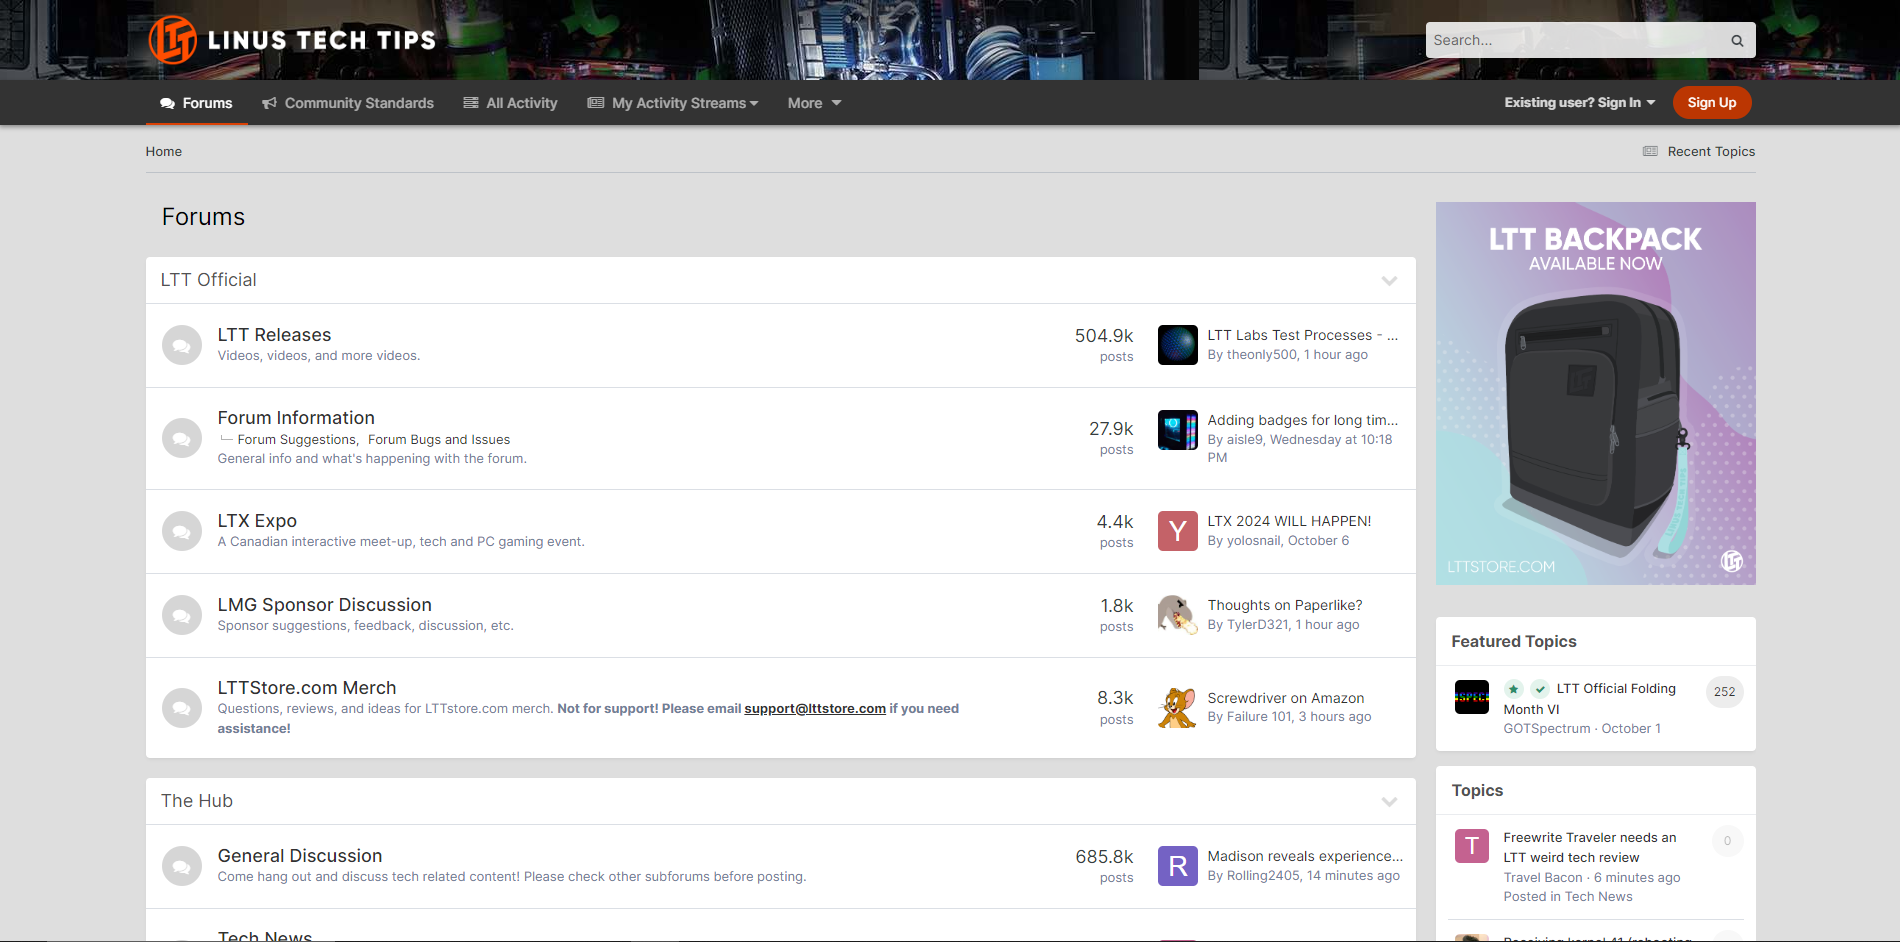
\includegraphics[width=0.7\textwidth]{image.png}
    \caption{Imagem do site de referencia}
    \label{fig:imagem}
  \end{figure}

  neste momento ja iniciamos algumas coisas desse projeto, por exemplo a parte de models, ja fizemos algumas classes. como demostrado na figura 2

  \begin{figure}[h]
    \centering
    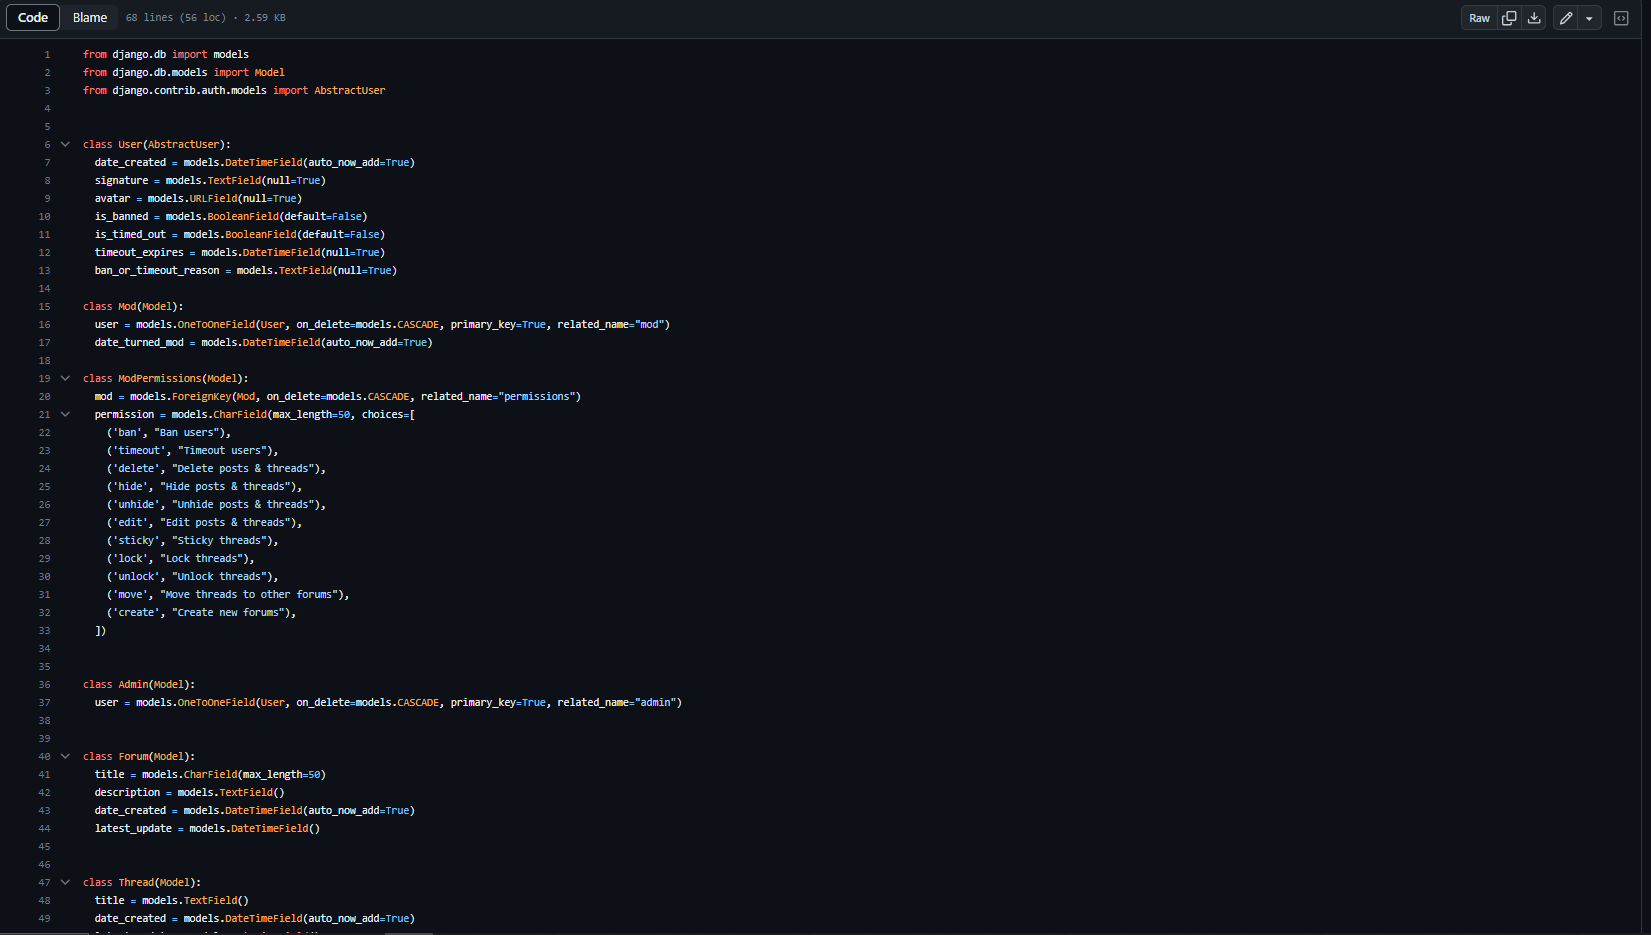
\includegraphics[width=0.7\textwidth]{image1.png}
    \caption{Imagem do arquivo models.py}
    \label{fig:imagem}
  \end{figure}

  Grupo 4 - \\
  André Plancha, 105289 \\
  Allan Kardec Rodrigues, 103380 \\
  Rui Chaves, 104914

\end{document}
